\documentclass[a4paper]{article}

% Options possibles : 10pt, 11pt, 12pt (taille de la fonte)
%                     oneside, twoside (recto simple, recto-verso)
%                     draft, final (stade de développement)

\usepackage[utf8]{inputenc}   % LaTeX, comprends les accents !
\usepackage[T1]{fontenc}      % Police contenant les caractères français
\usepackage[francais]{babel}  % Placez ici une liste de langues, la
                              % dernière étant la langue principale

\usepackage[a4paper]{geometry}% Réduire les marges
% \pagestyle{headings}        % Pour mettre des entêtes avec les titres
                              % des sections en haut de page

% Ajout de paquets perso
\usepackage{graphicx}
\usepackage{url}

\title{Structuration de la connaissance en Statistiques sur Wikipédia}           % Les paramètres du titre : titre, auteur, date
\author{Framartin}
\date{}                       % La date n'est pas requise (la date du
                              % jour de compilation est utilisée en son
			      % absence)

\sloppy                       % Ne pas faire déborder les lignes dans la marge

\begin{document}

\maketitle                    % Faire un titre utilisant les données
                              % passées à \title, \author et \date

\begin{abstract}
Nous avons étudié la façon dont est structurée la connaissance sur Wikipédia dans le domaine des statistiques en analysant les liens hypertextes entre pages de l'encyclopédie en rapport avec ce domaine. Nous construisons un graphe orienté où chaque lien représente une notion de référence que le lecteur est invité à consulter. Étudier cette problématique via le prisme de l'analyse de réseau, nous autorise à appréhender à la fois les parcours possibles de lecteurs au sein de ce site web (\textit{web mining}), mais surtout à la manière dont la connaissance est divisée en articles interdépendants se faisant référence asymétriquement. Cette approche nous permet de déterminer les sous-domaines et les sujets fondamentaux ou périphériques en statistiques, notamment via les notions de \textit{hubs}, autorité, centralité, et cohésion.
\end{abstract}

%\tableofcontents              % Table des matières

% \part{Titre}                % Commencer une partie...

\section{Introduction}               % Commencer une section, etc.

Wikipédia a connu depuis sa création une croissance impressionnante pour devenir le 6\ieme{} site web le plus visité au monde\footnote{\url{https://fr.wikipedia.org/wiki/Wikip\%C3\%A9dia}} avec plus de 8,5 millions de pages vues par heures en octobre 2014 pour la seule langue anglaise\footnote{\url{https://stats.wikimedia.org/FR/Sitemap.htm}}. Mais surtout Wikipédia est la plus grosse base d'informations populaire sur Internet. Or un des principes fondamentaux du web est la notion d'hyperlien, c'est à dire des liens vers d'autres pages web. Ceci nous invite à analyser ces liens qui sur Wikipédia prennent un sens particulier~: ils représentent des références d'un sujet donné.

La question qui se pose alors est de savoir comment une connaissance complexe, c'est à dire nécessitant des acquis pour la comprendre, va être divisée en différents articles cohérents et liés entre eux afin qu'un lecteur puisse trouver l'information qui lui manque. Cette information nous permet d’appréhender une forme de «~hiérarchie~» dans la connaissance en statistiques, dans le sens où certains sujets seront des fondamentaux universels et d'autres seront plus spécialisés dans un domaine. Cette problématique peut donc bien être analysée via le prisme de l'analyse statistique de réseau.

Nous pouvons construire un réseau sur la base d'un graphe orienté où les sommets sont des articles de Wikipédia et où un arc représente un lien hypertexte d'un article vers un autre article. Vu le nombre très élevé de pages sur Wikipédia, nous réduisons l'analyse aux articles appartenant au champ de la statistique. Ce réseau représente donc un ensemble interdépendant de références entre partie de la connaissance en statistiques.

Nous chercherons à déterminer quels sont les sujets et sous-domaines de la statistiques que l'on peut considérer comme universellement fondamentaux, périphériques, ou indépendants. Nous nous intéresserons aux articles les plus cités, ceux qui le sont le moins, aux plus centraux, et à l’existence de sous-ensembles cohérents, c'est à dire très référencés entre eux mais qui sont assez indépendants des autres articles. Ces questions seront étendus aux interdépendances des catégories de la statistique.

\section{Données} 

Afin d'apporter un éclairage à cette question, nous avons extrait les données suivantes~:
\begin{itemize}
    \item la liste des catégories d'articles de Wikipédia en rapport avec les statistiques ;
    \item la liste des articles de Wikipédia en rapport avec les statistiques ;
    \item pour chaque article sélectionné :
        \begin{itemize}
            \item l'ensemble des liens hypertextes vers un autre article de Wikipédia en rapport avec les statistiques ;
            \item sa taille en octet ;
            \item les catégories en rapport avec les statistiques auxquelles elle appartient.
        \end{itemize}
    \item la liste des articles de Wikipédia en rapport avec les Statistiques marqué comme «~ébauche~» ou nécessitant une relecture experte.
\end{itemize}

Nous nous sommes exclusivement intéressés à la version anglaise de Wikipédia qui est la plus complète dans ce domaine.


Pour extraire les données nécessaires à cette analyse, nous avons écrit un (long) script en Python 2.7. L'intégralité des codes et des données sont disponibles publiquement sur GitHub\footnote{Le dépôt git utilisé est disponible à cette adresse \url{https://github.com/Framartin/wikipedia_network_analysis}}. Le code en Python et R sont documentés et mis à disposition sous licence MIT.

Nous extrayons les données listées précédemment en utilisant l'API de MediaWiki (le moteur de Wikipédia) qui permet d'accéder à l'information voulue à partir de requêtes. Cela permet d'éviter de \textit{parser} l'intégralité de l'énorme base de données de Wikipédia. Pour ce faire, nous avons utilisé l'excellent tutoriel en Python écrit par Brian Keegan\footnote{Disponible sur GitHub sous licence MIT à cette adresse \url{https://github.com/brianckeegan/Wikipedia-Network-Analysis}}.


Nous allons détaillé l'extraction de données afin de comprendre les intérêts et les limitations de la méthode choisie.

    \subsection{Extraction des pages en rapport avec la statistique}

La liste des articles appartenant au champ de la statistique ont été récupéré à partir de deux pages qui listent les articles les plus importants de ce domaine\footnote{\url{https://en.wikipedia.org/wiki/List_of_statistics_articles} et \url{https://en.wikipedia.org/wiki/Outline_of_statistics}}. Nous enlevons ces deux articles afin d'éviter d'introduire un biais dans notre réseau (si nous les laissons le diamètre de notre réseau est borné à 5). Ce réseau est constitué par 2553 nœuds et 143394 liens.

Wikipédia est organisé en plusieurs espaces de noms\footnote{\url{https://fr.wikipedia.org/wiki/Aide:Espace_de_noms}}. Ce sont les préfixes des noms de pages qui permettent de classifier toutes les pages en différents types : Principal (0), Discussion (1), Utilisateur (2), Portail (100), Aide (12), Catégorie (16), etc. Ici, nous nous limitons à l'espace de noms principal (option \textit{plnamespace=0} de la requête), qui correspond à 99\% des articles de Wikipédia que nous lisons habituellement. On évite ainsi les liens vers des pages inutiles dans notre analyse\footnote{Comme \url{http://en.wikipedia.org/wiki/Special:PrefixIndex/Ubuntu}}. Nous avons également enlevé les pages dont le nom commence par \textit{List(s) of} ou \textit{Outline(s)} qui contiennent généralement un nombre très importants de liens, et ne correspondent pas à une organisation du savoir comme nous l'entendons.

Notons que nous avons également essayé d'extraire les nœuds de notre réseau via la catégorie \textit{Statistics} de Wikipédia\footnote{\url{https://en.wikipedia.org/wiki/Category:Statistics}}. Cependant les catégories de Wikipédia ne sont pas conçues pour cela, car ce ne sont pas des arbres : un article peut appartenir à plusieurs catégories, et une sous-catégorie peut appartenir à plusieurs catégories. Nous avons cependant extrait les sous-catégories sur 2 niveaux, et les pages appartenant à cette liste de sous-catégories de \textit{Statistics}. Mais outre le fait qu'il manquait 99 articles importants que la méthode précédente capturait, nous avions dans les pages des sujets qui ne concernaient pas le champ de la statistique comme nous le voulions. Par exemple, la catégorie \textit{Nomenclature of Territorial Units for Statistics de Statistics} appartenant à la sous-catégorie \textit{Nomenclature of Territorial Units for Statistics de Statistics} de \textit{Statistics}, nous conduisait à avoir \textit{Local administrative unit}, ou encore la \textit{Demography} aboutissait à \textit{Demographics by country} qui inclue des articles décrivant la démographie de nombreux pays. Le principe de parcimonie, nous conduit donc à sélectionner la première méthode qui, si elle est plus restrictive, semble plus pertinente.

    \subsection{Extraction des hyperliens}

Une fois la liste des pages définies, nous pouvons pour chacune d'entre-elle déterminer les liens vers les pages de Wikipédia. Nous gardons ensuite que celles appartenant à notre sélection de pages et à l'espace de noms principal. Notons que pour cette opération, nous passons par l'option de l'API de génération d'une sélection de pages Web, ce qui nous permet de suivre les redirections. En effet, il existe sur Wikipédia des pages de redirection, qui n'ont aucun contenu mais qui servent à orienter l'utilisateur vers une autre page\footnote{Ce qui est utile pour les concepts ayant plusieurs dénominations~: \url{https://en.wikipedia.org/wiki/Wikipedia:Redirect}}. Nous faisons attention de bien utiliser l'option \textit{redirects} de l'API afin que les liens pointant vers des pages de redirection soient remplacés par le nom de la page finale (par exemple \textit{Time series analysis} redirige automatiquement vers \textit{Time series}). Il est pertinent de procéder de la sorte car par défaut Wikipédia redirige automatiquement les navigateurs, et l'utilisateur n'a donc pas à cliquer pour aboutir sur la bonne page. Ainsi si une page renvoie vers \textit{Time series analysis}, nous récupérons le lien vers \textit{Time series}.

Chaque requête renvoie un nombre de liens bornés par une limite (10 par défaut que l'on peut augmenter jusqu'à 500 avec l'option \textit{pllimit}). Le module \textit{wikitools} s'occupe pour nous d'envoyer autant de requêtes que nécessaire afin d'avoir la totalité des liens d'une page.

Le fait de passer par l'API est pratique mais pose un problème : les articles incluent parfois des \textit{Templates}\footnote{\url{https://en.wikipedia.org/wiki/Help:Template}} utilisés pour orienter le lecteur vers des articles du domaine concerné à la fin de la page. Cependant ceux-ci sont inclus dans les liens que nous extrayons. C'est une limitation de notre façon d'extraire les données, mais la seule solution pour extraire uniquement les liens présents dans le corps d'un article serait de \textit{parser} l'intégralité d'un \textit{dump} des pages de Wikipédia, c'est à dire plusieurs Teraoctets de fichiers texte, ce qui dépasse le cadre de ce cours. Il faudra donc garder à l'esprit que nous avons dans notre réseau plus de liens que nécessaire. La seule chose facile que nous ayons pu faire c'est retirer les boucles (\textit{loop}), c'est à dire les liens vers la même page inclus à cause des \textit{templates}.

    \subsection{Extraction d'informations supplémentaires}

L'API nous autorise également à récupérer certaines caractéristiques des pages, ce que nous utilisons pour avoir leur taille en octets. Nous avons aussi pu obtenir la liste des articles de la statistique et de l'économétrie marqués comme ébauche\footnote{\url{https://en.wikipedia.org/wiki/Wikipedia:Stub}}, c'est à dire les articles trop courts pour apporter un savoir encyclopédique sur un sujet, ou ceux nécessitant une relecture experte. 

    \subsection{Création d'un deuxième réseau agrégé}
    \label{title:reseau-agg}

Afin de créer en plus un réseau agrégé, nous avons extrait les catégories à laquelle appartienne chaque page. Nous ne gardons que les catégories en rapport avec la statistique grâce à la liste des catégories de la statistique\footnote{\url{https://en.wikipedia.org/wiki/Wikipedia:WikiProject_Statistics/List_of_statistics_categories}}. Ce réseau est basé sur un graphe dirigé dans lequel les sommets sont des sous-domaines de la statistique, et les arrêtes les hyperliens entre articles appartenant à ces sous-champs. Les liens sont pondérés et chaque poids est défini par la somme du nombre de liens depuis tous les articles d'un domaine vers tous les articles d'un autre domaine. La taille de chaque nœud correspond au nombre d'articles de ce domaine. Ce réseau n'est pas simple car il peut contenir des boucles. Ce réseau est constitué par 199 nœuds et 22933 liens.

Dans notre cas, seulement 148 pages n'ont aucune catégorie. Elles sont retirées du réseau. Une page de Wikipédia appartient souvent à plusieurs catégories. Dans l'agrégation, nous avons choisi de dupliquer les liens d'une page pour chaque catégorie à laquelle elle appartient. Ceci ne nous semble pas problématique dans la mesure où nous nous intéressons à la détermination des domaines des statistiques référents ou référencés par un domaine donné.


\section{Analyse des références entre articles} 

Nous nous intéressons dans un premier temps à l'analyse du réseau des articles en rapport avec la statistique, afin d'étudier les relations de référence entre eux. Ce réseau est composé 2553 sommets reliés par 143394 arrêtes et est simple.

Le première question que l'on peut se poser est de savoir si le nombre de références présentes dans un article et le nombre d'articles référençant une page donnée sont uniformément répartis. Autrement dit, y-a-il une hétérogénéité dans la distribution des liens, ou est-ce que le réseau est plutôt homogène ? Cette question est fondamentale car elle nous renseigne sur l'organisation de la connaissance~: l'encyclopédie en ligne est-elle composée par quelques articles faisant autorité et une majorité d'articles peu cités, ou par une découpe homogène des sujets portant sur les statistiques ?

\begin{figure}[h!]
   \centering
   \caption{\label{hist-in-deg} Histogramme des degrés entrants des sommets}
   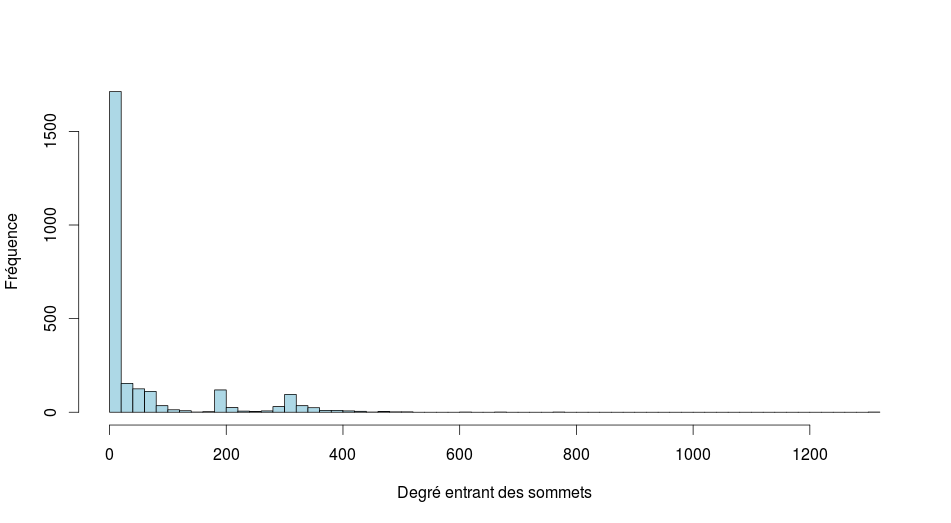
\includegraphics[scale=0.40]{../images/vertex_in_dist}
\end{figure}

\begin{figure}[h!]
   \centering
   \caption{\label{log-log-deg} Probabilités empiriques des degrés entrants et sortants}
   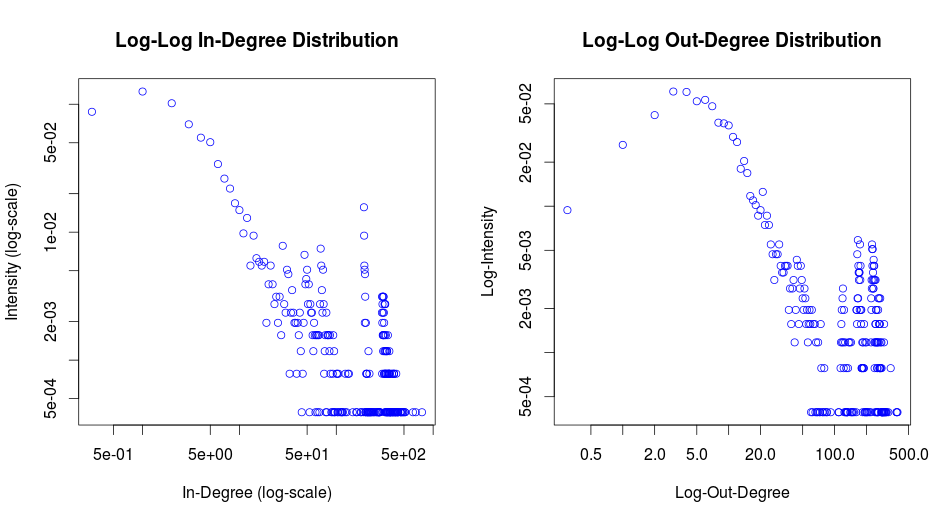
\includegraphics[scale=0.35]{../images/log-log-dist-deg}
\end{figure}


Premièrement, étudions la distribution des liens entrants, c'est à dire des degrés entrants des sommets. La figure \ref{hist-in-deg} représente l'histogramme des degrés entrants des sommets. On peut observer qu'il y a une grande disparité du nombre de liens entrants vers les articles, c'est à dire, que la notion de référence n'est pas également distribuée entre les articles de statistiques sur Wikipédia~: certains sont très fondamentaux dans ce domaine et d'autres beaucoup moins. En effet, le degré entrant maximum est de $1316$, alors que l'on peut voir qu'une très grande partie des articles ne sont très peu cités. De plus, l'écart est très important entre la médiane, égale à 6, et la moyenne, égale à $56,17$. Ceci nous indique une forte dispersion des articles référents en statistique. 

\begin{figure}[h!]
   \centering
   \caption{\label{hist-out-deg} Histogramme des degrés sortants des sommets}
   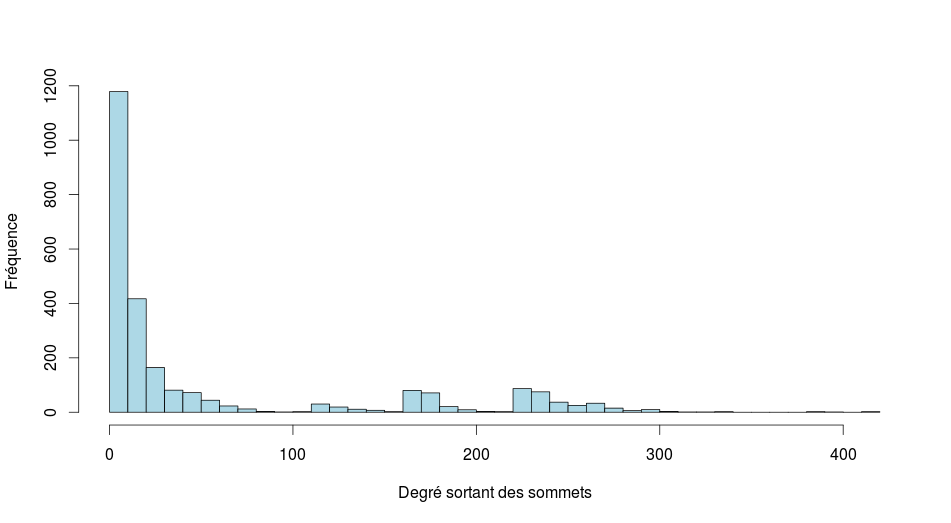
\includegraphics[scale=0.40]{../images/vertex_out_dist}
\end{figure}

Il est également intéressant d'étudier plus en détails cet histogramme. Les noms des articles ayant plus 450 liens entrants sont reportés dans le tableau \ref{tab-deg-in}. On remarque que 4 articles ont un degré très élevé : \textit{Statistics}, et 3 notions fondamentales (\textit{Probability distribution}, \textit{Variance} et \textit{Normal distribution}). Un deuxième ensemble d'articles se dessine entre 450 et 600 degrés, et correspondent à des sous-domaines fondamentaux (\textit{Time series}, \textit{Regression analysis}, \textit{Linear regression}, et \textit{Econometrics}), des outils très utilisés (\textit{Kolmogorov–Smirnov test}, \textit{Mean}, \textit{Maximum likelihood}, \textit{Standard deviation}) et des notions fondamentales (\textit{Exponential family}). Un «~pic~» se situe entre 250 et 450 degrés et se constitue de beaucoup de sujets différents : méthodes, modèles, notions probabilistes, données, champ des statistiques, visualisation de données. Cependant il est très intéressant de constater que le «~pic~» entre 150 et 250 degrés et quasiment exclusivement constitué de pages décrivant une loi probabiliste. Il serait intéressant d'explorer plus en détails les raisons de cette similarité. Notons cependant que les distributions ne sont pas citées toutes le même nombre de fois.

\begin{table}[ht]
\centering
\caption{\label{tab-deg-in} Articles ayant plus de 450 liens entrants}
\begin{tabular}{rr}
  \hline
 Titre & Degré entrant \\ 
  \hline
Statistics & 1316 \\ 
  Probability distribution & 767 \\ 
  Variance & 661 \\ 
  Normal distribution & 619 \\ 
  Exponential family & 513 \\ 
  Kolmogorov–Smirnov test & 512 \\ 
  Time series & 495 \\ 
  Regression analysis & 492 \\ 
  Linear regression & 479 \\ 
  Mean & 476 \\ 
  Econometrics & 464 \\ 
  Maximum likelihood & 462 \\ 
  Standard deviation & 460 \\ 
   \hline
\end{tabular}
\end{table}

La distribution des liens sortants n'est pas homogène dans notre réseau, comme le montre l'histogramme en figure \ref{hist-out-deg}. Les articles ayant les plus hauts degrés sortants concernent des lois probabilistes construites à partir d'autres lois (\textit{Student's t-distribution}, \textit{Noncentral t-distribution}, \textit{Skew normal distribution}, \textit{Generalized normal distribution}), ce qui suggère que ces sujets complexes et fondamentaux utilisent une grande quantité de références. On retrouve exclusivement des pages détaillant des distributions de lois dans le «~pic~» sur l'histogramme entre 160 et 220 degrés. Ce qui semble suggérer une façon identique d'organiser le savoir sur ces concepts probabilistes.

La figure \ref{hex-deg-nei} représente la moyenne des degrés des voisins par rapport au degré d'une page avec une représentation conçue pour les fortes densités dans laquelle le plan est découpé en hexagones. Notons que les degrés représentés ici sont les sommes des degrés entrants et sortants. On peut remarquer que les articles ayant un très faible degré sont connectés soit avec des articles ayant un degré très élevé, soit avec des articles ayant un degré très faible. Plus le degré d'un article devient grand, plus ses voisins semblent similaires en terme de degré. Notons enfin que les articles avec un degré élevé semble avoir des voisins de degrés élevés et approximativement égal. Ainsi, les articles ayant des degrés élevés que l'on a identifié comme fondamentaux sont connectés entre eux et semble constituer un cœur du réseau dense.

\begin{figure}[h!]
   \centering
   \caption{\label{hex-deg-nei} Degrés des voisins en fonction des degrés des sommets (log-log)}
   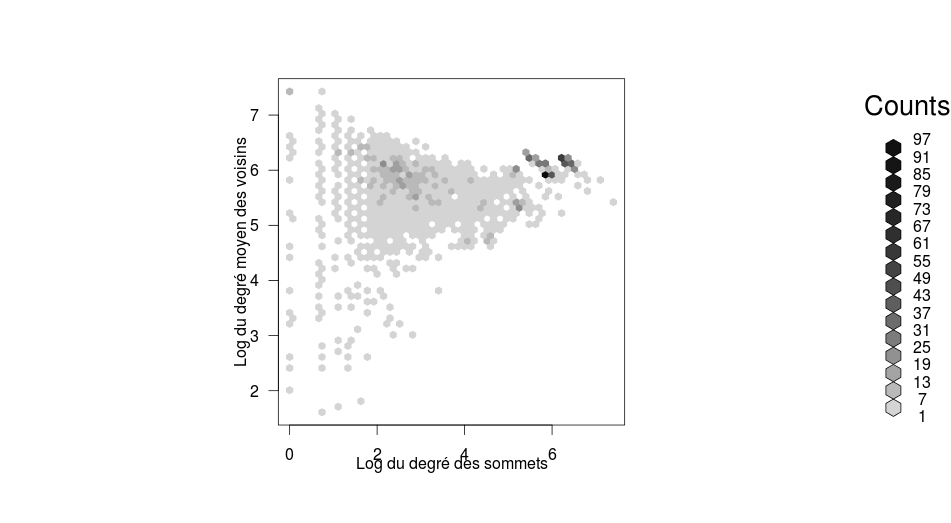
\includegraphics[scale=0.40]{../images/hex-deg-nei}
\end{figure}

La connaissance dans le domaine statistique semble également dense pour d'autres raison. Ainsi la réciprocité de notre graphe est de $0,551$ et la densité de $0,022$. De plus, on compte $64420$ dyades asymétriques et $39487$ dyades réciproques. On peut s'interroger sur la pertinence des liens mutuels, dans le sens où des références cycliques n'apportent pas d'informations. Le diamètre du réseau n'est que de $8$, celui ci est donc resserré. Avec un diamètre et une longueur moyenne des plus courts chemins (égale à $2,922$) peu élevés, et un coefficient de \textit{clustering} élevé ($0,664$), nous nous retrouvons dans une configuration de type \textit{small world}. Ce qui nous montre que la connaissance en statistique est assez unie.

La détection de communauté basée sur les valeurs propres de la matrice modulaire (\textit{modularity matrix}) aboutit à 16 communautés dont 6 à un seul sommet, 4 à 2 sommets, 1 à 367, 1 à 18, 1 à 55, 1 à 90, 1 à 521 et un autre à 1470 sommets. Cela semble indiquer la nature dense du corps principal des statistiques. Notons que celui à 367 sommets regroupe essentiellement des articles sur des lois probabilistes, celui à 521 sommets de la statistique mathématique et celui à 90 sommets des logiciels. Ainsi on aperçoit des sous-champs gravitant autour de la statistique qui sont fondamentaux (probabilité et statistique mathématique) ou utiles (informatique). Et si ces derniers sont dans l'absolu beaucoup reliés à la statistique, ils le sont relativement moins que son cœur.

La corrélation entre la taille en octets des articles et leurs degrés entrants de $0,303$ et la figure \ref{size-deg-in} semblent nous indiquer que les longs articles sont ceux qui font le plus références. Cependant, amendons ce propos en ajoutant que si l'on observe cette tendance globale, pour un degré donné, il existe des tailles d'articles très différentes. Ainsi des articles ayant un faible degré entrant peuvent être longs, et ceux ayant un degré très élevé ont une taille sont tous supérieurs à une taille minimum. Ainsi la taille joue un rôle mais n'est pas déterminante dans la relation de référence.

\begin{figure}[h!]
   \centering
   \caption{\label{size-deg-in} Degrés entrants en fonction de la taille des pages (log-log)}
   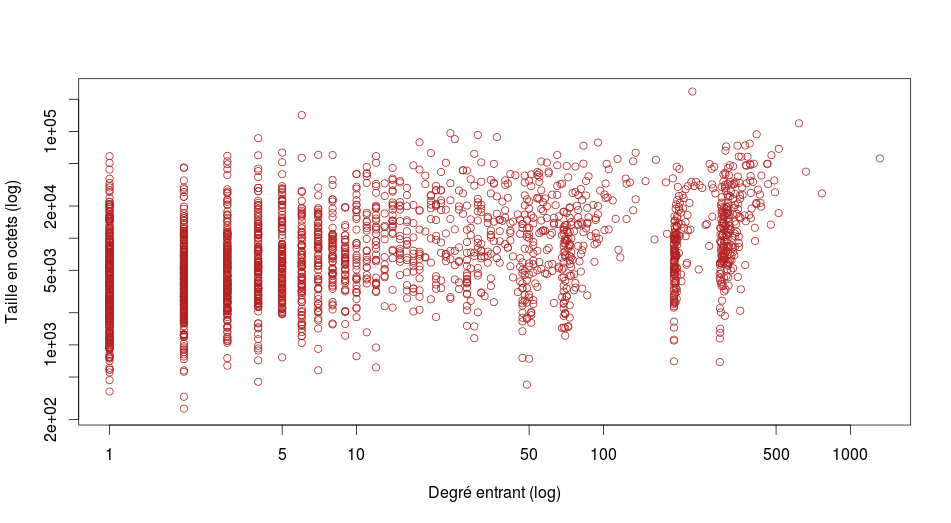
\includegraphics[scale=0.40]{../images/size_d_in}
\end{figure}

La connaissance sur Wikipédia s'élabore également par la classification d'articles comme ébauches ou nécessitant une relecture experte. On peut se demander si ces articles font référence (car ils bénéficient d'une attention particulière) ou au contraire s'ils ne sont nouveaux et donc pas centraux. La moyenne et la médiane des degrés entrants des ébauches sont respectivement de $9,75$ et $2$, alors que pour les autres articles elles sont égales à $61,13$ et $7$. Les différences sont donc très importantes et un test bilatéral de Student nous confirme que la différence des deux moyennes est significativement différente de 0 (p-value $< 2.2e^{-16}$). Cependant les articles marqués comme nécessitant une relecture experte ont eux des degrés entrants beaucoup plus proches des autres articles (moyenne de $58,14$ contre $56,12$, et médiane de $5$ contre $6$). Avec une p-valeur de $0.89$ le test de Student arrive à la conclusion que les deux moyennes se sont pas significativement différentes. Il semble donc que les ébauches sont beaucoup moins centrales dans la connaissance en statistiques, et que les articles nécessitant une relecture experte sont quant à eux autant référant que les autres.


\section{Analyse des références entre catégories} 

Dans un deuxième temps, il semble intéressant d'agréger ce réseau à des fins d'interprétation et de visualisation. En effet le réseau précédant comporte trop de sommets et d’arrêtes pour être lisible. Nous avons donc créé un réseau agrégé comme expliqué dans la partie \ref{title:reseau-agg}, c'est à dire entre catégories des statistiques.

Cependant ce réseau comporte encore 199 catégories et 22933 liens. Malgré divers essais d'agencement (\textit{layout}), la visualisation n'était pas facilement lisible. Vu le nombre de liens très petits entre certaines catégories et l'existence de catégories n'ayant que très peu d'articles (cf. figure \ref{hist-agg}), nous avons choisi de réduire la visualisation à un sous-réseau. Nous avons pris les catégories ayant au moins 60 articles, ce qui revient à choisir les 21 plus gros nœuds. De plus, à des fins de lisibilité, nous conservons les liens ayant un poids, c'est à dire un nombre de liens entre les articles appartenant à ses catégories, supérieur à 364. Ce qui nous amène à une représentation d'un réseau à 111 liens.

\begin{figure}[h!]
   \centering
   \caption{\label{hist-agg} Histogrammes des poids des liens du réseau et de la taille des catégories}
   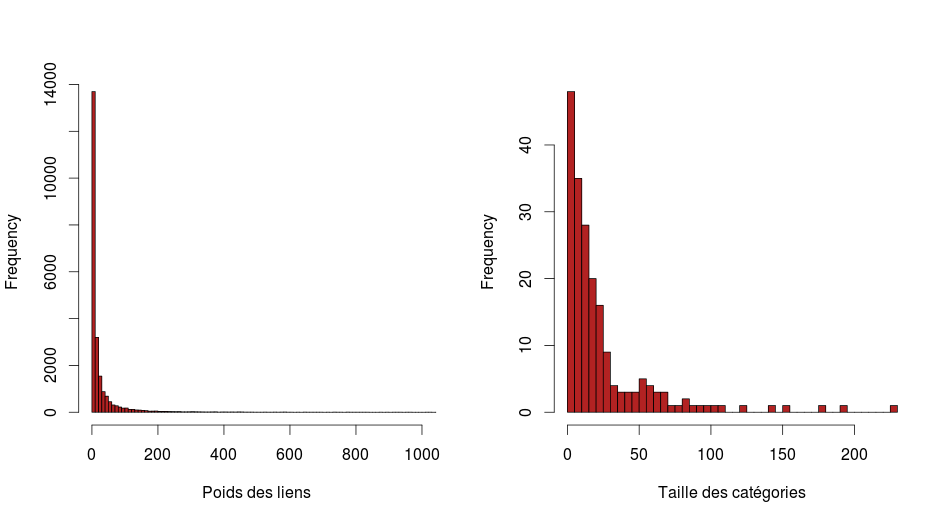
\includegraphics[scale=0.35]{../images/hist-agg}
\end{figure}

À partir de ce réseau, nous avons testé différentes dispositions, comme la méthode de Fruchterman et Reingold, la disposition en cercle, ou la méthode DrL, mais l'agencement le plus lisible était celui donné par l'approche de Kamada et Kawai. Sur la figure \ref{viz-cat}, la taille des sommets correspond au nombre d'articles d'une sous-catégorie des statistiques et la largueur des flèches représente le poids des arcs.

\begin{figure}[h!]
   \centering
   \caption{\label{viz-cat} Visualisation des liens entre catégories de la statistique}
   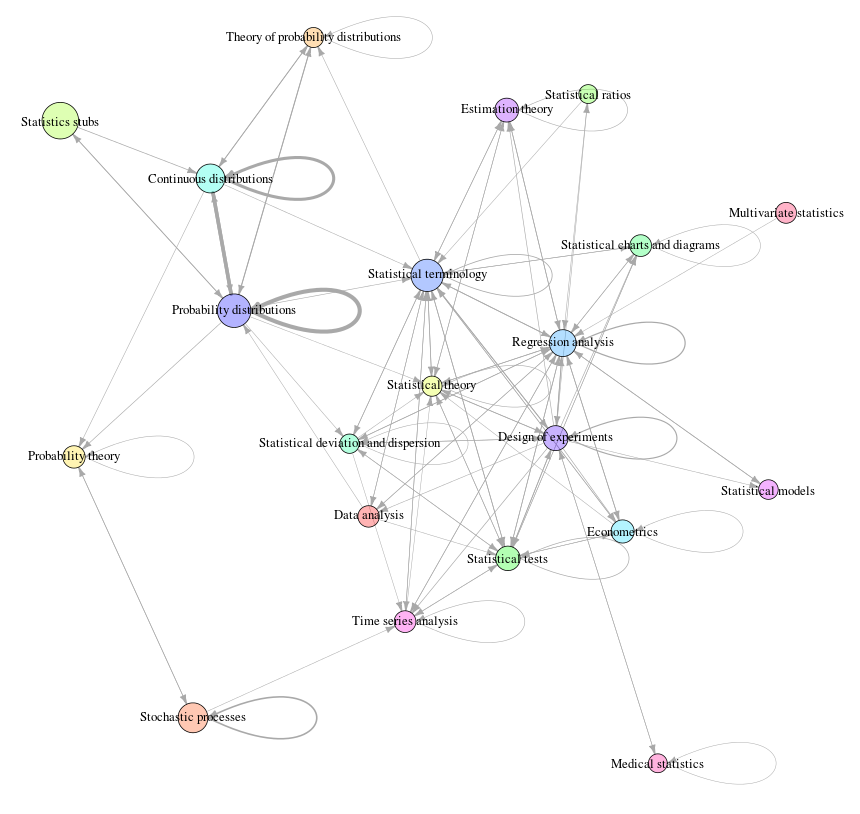
\includegraphics[scale=0.5]{../images/categories2}
\end{figure}

Il est intéressant d'analyser la relation entre les catégories relevant de sujets théoriques et les domaines de statistiques appliquées. Par exemple, l'économétrie utilise ses propres références mais aussi celles des tests, des régressions, de la théorie statistique, ou des plans d'expérience. La catégorie \textit{Medical Statistics}, qui est un champ d'application particulier, s'appuie sur les plans d'expérience, mais la réciproque est aussi vrai. Ainsi on peut observer des allers-retours entre la théorie non-probabiliste et les applications en statistiques. Quand à la théorie probabiliste, elle se fait beaucoup référence elle-même et est quelque peu à part du réseau, tout en y étant connecté. Cela correspond bien au fait que les fondamentaux des statistiques sont probabilistes, mais qu'inversement la théorie probabiliste reste assez indépendantes des statistiques pures.
 
On peut également constater le nombre important de catégories qui référencent la terminologie statistique, et nous indique que sur Wikipédia les liens hypertextes ne servent pas uniquement à donner des approfondissements sur des sujets fondamentaux, mais également à expliciter du vocabulaire technique.

La densité de liens au centre du réseau montre l'interdépendance forte entre les différents champs de la statistique, ainsi l'analyse de données, les tests statistiques, les plans d'expérience, les régressions, la théorie statistique sont des sujets qui se font mutuellement référence. Cela correspond au fait que l'on ne peut maîtriser une partie d'un de ces domaines sans connaître aucun des autres.


\section{Conclusion} 

Nous avons donc pu voir que si les statistiques sont un domaine très dense et composé de sous-champs très interdépendants, certains sont plus périphériques que d'autres, comme les mathématiques fondamentales les probabilités ou l'informatique. L'analyse en terme de réseau nous a conduit à identifier certaines notions fondamentales. Cette approche nous renseigne à la fois sur la structuration de la connaissance sur le média particulier qu'est Wikipédia, mais aussi plus généralement sur les statistiques.

Il serait intéressant de poursuivre cette analyse en extrayant les données directement depuis les sauvegardes de Wikipédia afin de ne récupérer que les liens hypertextes présents dans le corps des articles. Ainsi nous pourrions étudier l'effet qu'a eu l'inclusion des \textit{templates} sur la structure du réseau, en s'intéressant aux variations du diamètre, de la réciprocité, des degrés entrants, etc.

% \appendix                   % Commençons les annexes

% \section{Titre}             % Annexe A

% \section{Titre}             % Annexe B

% \listoffigures              % Table des figures

% \listoftables               % Liste des tableaux

\end{document}

